\documentclass[12pt,a4paper]{article}
\usepackage[utf8]{inputenc}
\usepackage[spanish]{babel}
\usepackage{geometry}
\usepackage{amsmath}
\usepackage{amssymb}
\usepackage{booktabs}
\usepackage{graphicx}
\usepackage{enumitem}
\usepackage{tikz}
\usepackage{float}
\usepackage{xcolor}
\usepackage{hyperref}
\geometry{margin=2.5cm}

\hypersetup{
    colorlinks=true,
    linkcolor=blue,
    citecolor=blue,
    urlcolor=blue
}

\begin{document}

%============================================================================
% ALTERNATIVA A: UASB + FILTRO PERCOLADOR + UV
% Memoria de Cálculo
%============================================================================
\newpage
\section{Alternativa A: Tratamiento Anaerobio-Aerobio con UASB y Filtro Percolador}

La presente alternativa propone un esquema de tratamiento que combina procesos anaerobios y aerobios para lograr la remoción de contaminantes de manera eficiente y con bajo consumo energético. El tren de tratamiento completo comprende: rejillas y desarenador para el pretratamiento, reactor UASB para el tratamiento primario anaerobio, filtro percolador para el tratamiento secundario aerobio, sedimentador secundario para la separación de sólidos biológicos, y finalmente desinfección UV antes del vertimiento.

\subsection{Canal de Desbaste con Rejillas}

Las rejillas constituyen la primera barrera de protección del sistema, reteniendo sólidos gruesos como plásticos, ramas y papel que podrían dañar equipos o causar obstrucciones en tuberías aguas abajo. El diseño hidráulico de esta unidad debe garantizar velocidades suficientes para arrastrar sólidos sedimentables, pero no tan elevadas que dificulten el paso del agua a través de las barras.

Según los criterios establecidos por Metcalf y Eddy \cite{metcalf2014}, las velocidades de diseño en canales con rejillas deben mantenerse entre 0,40 y 0,60 m/s. Para este proyecto se adopta un valor intermedio de 0.50 m/s, lo cual resulta apropiado considerando el caudal de diseño. El tirante hidráulico se establece en 0.40 m, valor que permite una velocidad de flujo uniforme en la sección del canal y evita la sedimentación de sólidos orgánicos antes de la rejilla, según los criterios de Metcalf y Eddy \cite{metcalf2014}.

La pérdida de carga en rejillas limpias se calcula mediante la fórmula de Kirschmer (1926), que relaciona la geometría de las barras con las características del flujo. Los parámetros que determinan esta pérdida son: el espaciado entre barras ($b$), el espesor de las barras ($w$), la velocidad del flujo ($v$) y el ángulo de inclinación ($\theta$):

\begin{equation}
h_L = \beta \cdot \left(\frac{w}{b}\right)^{4/3} \cdot \frac{v^2}{2g} \cdot \sin\theta
\end{equation}

\textit{Donde:}
\begin{itemize}[noitemsep,leftmargin=2em]
    \item[$h_L$] = Pérdida de carga en rejillas limpias (m)
    \item[$\beta$] = Factor de forma de la barra (2,42 para barras rectangulares)
    \item[$w$] = Espesor de la barra (10 mm)
    \item[$b$] = Espaciado entre barras (15 mm)
    \item[$v$] = Velocidad del flujo en el canal (m/s)
    \item[$g$] = Aceleración de la gravedad (9,81 m/s²)
    \item[$\theta$] = Ángulo de inclinación de las barras (60°)
\end{itemize}

El caudal de diseño por línea es 5.0 L/s. La sección transversal del canal se determina aplicando la ecuación de continuidad:

\begin{equation}
A_{canal} = \frac{Q}{v} = \frac{0.00500}{0.50} = 0.01000 \text{ m}^2
\end{equation}

\textit{Donde:}
\begin{itemize}[noitemsep,leftmargin=2em]
    \item[$A_{canal}$] = Sección transversal del canal (m²)
    \item[$Q$] = Caudal de diseño por línea (0.00500 m³/s)
    \item[$v$] = Velocidad de diseño adoptada (0.50 m/s)
\end{itemize}

Despejando el ancho del canal de la ecuación $A = b \times h$, con $h = 0.40$ m:

\begin{equation}
b = \frac{A_{canal}}{h} = \frac{0.01000}{0.40} = 0.025 \text{ m}
\end{equation}

\textit{Donde:}
\begin{itemize}[noitemsep,leftmargin=2em]
    \item[$b$] = Ancho teórico del canal (m)
    \item[$A_{canal}$] = Sección transversal del canal (0.01000 m²)
    \item[$h$] = Tirante hidráulico (0.40 m)
\end{itemize}

Este ancho teórico de 0.025 m es inferior al mínimo constructivo práctico. Se adopta un ancho de 0,60 m como dimensión mínima constructiva según criterios de OPS/CEPIS \cite{ops2005} y SENAGUA \cite{senagua2012}, que establecen un ancho mínimo de 0,60 m para permitir la operación adecuada, el acceso para limpieza y la aplicación de herramientas de mantenimiento. Verificando la velocidad real con este ancho:

\begin{equation}
v_{real} = \frac{Q}{A_{real}} = \frac{0.00500}{0.60 \times 0.40} = 0.021 \text{ m/s}
\end{equation}

\textit{Donde:}
\begin{itemize}[noitemsep,leftmargin=2em]
    \item[$v_{real}$] = Velocidad real verificada con ancho constructivo (m/s)
    \item[$Q$] = Caudal de diseño (0.00500 m³/s)
    \item[$A_{real}$] = Sección real con ancho constructivo adoptado (0.60 × 0.40 m²)
\end{itemize}

La velocidad real de 0.021 m/s es el resultado de adoptar el ancho mínimo constructivo. La pérdida de carga calculada con esta velocidad real resulta $h_L = 0.0027$ cm, menor al umbral de 15 cm que Metcalf y Eddy \cite{metcalf2014} indican como referencia para sistemas de limpieza mecánica.

La longitud de 2.0 m y el ancho de 0.60 m responden a criterios constructivos y operativos. El ancho de 0,60 m es la dimensión mínima constructiva según OPS/CEPIS \cite{ops2005} y SENAGUA \cite{senagua2012}, que permite la operación adecuada de la rejilla, el acceso para limpieza y la aplicación de herramientas de mantenimiento. La longitud contempla el espacio de la rejilla propiamente dicha más las zonas de transición necesarias para la operación.

\subsubsection{Verificación para Caudal Máximo Horario}

Se verifica el comportamiento hidráulico para el caudal máximo horario, aplicando un factor de pico típico de 2.5 sobre el caudal medio:

\begin{equation}
Q_{max} = 2.5 \times Q_{medio} = 2.5 \times 5.0 = 12.5 \text{ L/s}
\end{equation}

A caudal máximo, la velocidad horizontal resulta:

\begin{equation}
v_{max} = \frac{Q_{max}}{A_{real}} = \frac{12.500/1000}{0.60 \times 0.40} = 0.052 \text{ m/s}
\end{equation}

\textbf{Criterios de verificación de velocidad} (según Metcalf y Eddy \cite{metcalf2014}):

La velocidad calculada $v_{max} = 0.052$~m/s se evalúa según:

\begin{equation}
\text{Estado} = \begin{cases}
    \text{ÓPTIMO} & \text{si } v_{max} \leq 1.5 \text{ m/s} \quad \text{(sin riesgo)} \\
    \text{ACEPTABLE} & \text{si } 1.5 < v_{max} \leq 2.0 \text{ m/s} \quad \text{(monitoreo)} \\
    \text{NO ADMISIBLE} & \text{si } v_{max} > 2.0 \text{ m/s} \quad \text{(daño seguro)}
\end{cases}
\end{equation}

Con la velocidad calculada $v_{max} = 0.052$~m/s, es menor que el límite recomendado de 1,5~m/s para operación segura. Respecto a la pérdida de carga, el valor máximo de 0.0169~cm es menor que el umbral de 15~cm para limpieza manual aceptable.

\subsubsection{Resultados}

\begin{table}[H]
\centering
\caption{Verificación de criterios de diseño - Rejillas}
\begin{tabular}{lccc}
\toprule
Parámetro & Valor calculado & Criterio & Estado \\
\midrule
Velocidad de diseño & 0.50 m/s & 0,40 -- 0,60 m/s & Cumple \\
Velocidad real & 0.021 m/s & Ancho mínimo constructivo$^a$ & Aplicado \\
Pérdida de carga (Qmax) & 0.0169 cm & $<$ 15 cm & Cumple \\
Ancho constructivo & 0.60 m & $\geq$ 0,30 m & Cumple \\
\bottomrule
\end{tabular}
\small
$^a$ Para caudales pequeños (5 L/s) el ancho mínimo constructivo (0,60 m) domina sobre el criterio de velocidad.
\end{table}

\begin{figure}[H]
\centering
\begin{tikzpicture}[scale=1.0, line cap=round, line join=round]

% === SECCION TRANSVERSAL (izquierda) ===
\begin{scope}[xshift=-4.5cm]
    % Paredes del canal (gris claro)
    \fill[gray!20] (0,0) rectangle (3.6,1.5);
    % Borde del canal
    \draw[very thick] (0,0) rectangle (3.6,1.5);
    % Agua (azul muy claro)
    \fill[blue!10] (0.1,0.1) rectangle (3.5,1.0);
    % Linea de agua punteada
    \draw[blue, thick, dashed] (0.1,1.0) -- (3.5,1.0);
    % Barras de rejilla VERTICALES negras y gruesas
    \foreach \x in {0.4,0.8,1.2,1.6,2.0,2.4,2.8,3.2}{
        \draw[line width=2.5pt] (\x,0.1) -- (\x,1.4);
    }
    % Circulo azul con punto blanco (direccion perpendicular al plano)
    \fill[blue] (1.8,0.55) circle (0.18);
    \fill[white] (1.8,0.55) circle (0.06);
    % Cota del tirante (izquierda) con marcas de dimension
    \draw[thick] (-0.3,0.1) -- (-0.3,1.0);
    \draw[thick] (-0.4,0.1) -- (-0.2,0.1);
    \draw[thick] (-0.4,1.0) -- (-0.2,1.0);
    \node[left] at (-0.3,0.55) {$h = 0.40$~m};
    % Cota del ancho (abajo) con marcas de dimension
    \draw[thick] (0,-0.3) -- (3.6,-0.3);
    \draw[thick] (0,-0.4) -- (0,-0.2);
    \draw[thick] (3.6,-0.4) -- (3.6,-0.2);
    \node[below] at (1.8,-0.3) {$b = 0.60$~m};
    % Titulo
    \node[below, font=\bfseries] at (1.8,-0.9) {Seccion Transversal};
\end{scope}

% === VISTA LONGITUDINAL (derecha) ===
\begin{scope}[xshift=2cm]
    % Paredes del canal (gris claro)
    \fill[gray!20] (0,0) rectangle (6,1.2);
    % Borde del canal
    \draw[very thick] (0,0) rectangle (6,1.2);
    % Agua (azul muy claro)
    \fill[blue!10] (0.1,0.1) rectangle (5.9,1.1);
    \draw[thick] (0.1,0.1) rectangle (5.9,1.1);
    % Rejilla: barras verticales negras y gruesas
    \foreach \x in {1.7,1.85,2.0,2.15,2.3,2.45}{
        \draw[line width=2.5pt] (\x,0.1) -- (\x,1.1);
    }
    % Marco de la rejilla
    \draw[very thick] (1.6,0.05) rectangle (2.55,1.15);
    % Flechas de flujo AZULES con cabeza
    \draw[line width=2pt, blue!80!black] (0.4,0.6) -- (1.5,0.6);
    \fill[blue!80!black] (1.5,0.6) -- (1.25,0.45) -- (1.25,0.75) -- cycle;
    \draw[line width=2pt, blue!80!black] (2.7,0.6) -- (5.5,0.6);
    \fill[blue!80!black] (5.5,0.6) -- (5.25,0.45) -- (5.25,0.75) -- cycle;
    % Cota de longitud (abajo) con marcas de dimension
    \draw[thick] (0,-0.3) -- (6,-0.3);
    \draw[thick] (0,-0.4) -- (0,-0.2);
    \draw[thick] (6,-0.4) -- (6,-0.2);
    \node[below] at (3,-0.3) {$L = 2.0$~m};
    % Etiqueta Entrada
    \draw[thick] (0.1,1.5) -- (1.6,1.5);
    \node[above] at (0.85,1.5) {Entrada};
    % Etiqueta Rejilla
    \draw[thick] (1.6,1.5) -- (5.9,1.5);
    \node[above] at (3.75,1.5) {Rejilla};
    % Titulo
    \node[below, font=\bfseries] at (3,-0.9) {Vista Longitudinal};
\end{scope}

\end{tikzpicture}
\caption{Esquema del canal de desbaste con rejillas (dimensiones en metros)}
\label{fig:rejillas}
\end{figure}

Las dimensiones finales del canal con rejillas son: ancho 0.60 m, tirante 0.40 m y longitud 2.0 m. Se requieren dos unidades, una por cada línea de tratamiento.

\subsection{Desarenador de Flujo Horizontal}

El desarenador remueve partículas minerales (arena, grava) con diámetro superior a 0,20 mm mediante sedimentación gravitacional. Según Metcalf y Eddy \cite{metcalf2014}, los parámetros de diseño son: velocidad horizontal 0,25 - 0,30 m/s (máximo 0,30 m/s para evitar arrastre de sedimentos), tiempo de retención 30 - 60 s, y profundidad de flujo 0,75 - 2,0 m (OPS/CEPIS \cite{ops2005} permite valores menores en plantas pequeñas).

La profundidad total del canal incluye: profundidad útil de flujo (0.40~m), zona de almacenamiento de arena (0,25 - 0,30~m), y bordo libre (0,30~m).

El diseño del desarenador se fundamenta en la teoría de sedimentación discreta. Primero se calcula la velocidad de sedimentación de las partículas objetivo mediante la Ley de Stokes:

\begin{equation}
v_s = \frac{g \cdot (S_s - 1) \cdot d^2}{18 \cdot \nu}
\end{equation}

\textit{Donde:}
\begin{itemize}[noitemsep,leftmargin=2em]
    \item[$v_s$] = Velocidad de sedimentación (m/s)
    \item[$g$] = Aceleración de la gravedad (9.81 m/s²)
    \item[$S_s$] = Gravedad específica de la arena (2.65)
    \item[$d$] = Diámetro de la partícula (0.00020 m)
    \item[$\nu$] = Viscosidad cinemática del agua a 25.6°C ($8.3973e-07$ m²/s)
\end{itemize}

\begin{equation}
v_s = \frac{9.81 \times (2.65 - 1) \times (0.00020)^2}{18 \times 8.3973e-07} = 0.043 \text{ m/s}
\end{equation}

Con este valor de $v_s$ se determina la longitud teórica del desarenador mediante la ecuación de sedimentación tipo I:

\begin{equation}
L = \frac{H \cdot v_h}{v_s} = \frac{0.40 \times 0.30}{0.043} = 2.8 \text{ m}
\end{equation}

\textit{Donde:}
\begin{itemize}[noitemsep,leftmargin=2em]
    \item[$L$] = Longitud del desarenador (m)
    \item[$H$] = Profundidad útil (0.40 m)
    \item[$v_h$] = Velocidad horizontal adoptada (0.30 m/s)
\end{itemize}

La longitud teórica resultante (2.8~m) es adecuada para el caudal de diseño y se adopta como longitud de diseño.

El ancho del canal se determina por la ecuación de continuidad:

\begin{equation}
B = \frac{Q}{v_h \cdot H} = \frac{0.00500}{0.30 \times 0.40} = 0.042 \text{ m}
\end{equation}

\textit{Donde:}
\begin{itemize}[noitemsep,leftmargin=2em]
    \item[$B$] = Ancho teórico del canal (m)
    \item[$Q$] = Caudal de diseño (0.00500 m³/s)
\end{itemize}

El ancho teórico resulta inferior al mínimo constructivo. Se adopta 0.60 m según OPS/CEPIS \cite{ops2005} y SENAGUA \cite{senagua2012}, que establecen 0,60 m como ancho mínimo para operación y mantenimiento.

Verificando la velocidad horizontal real con el ancho adoptado:

\begin{equation}
v_{real} = \frac{Q}{B \cdot H} = \frac{0.00500}{0.60 \times 0.40} = 0.021 \text{ m/s}
\end{equation}

El tiempo de retención real resulta:

\begin{equation}
t_r = \frac{L}{v_{real}} = \frac{3.0}{0.021} = 144.0 \text{ s}
\end{equation}

\subsubsection{Verificación de Velocidad Crítica}

Para garantizar que la arena sedimentada no sea resuspendida por el flujo, se verifica que la velocidad horizontal del diseño sea menor que la velocidad crítica de resuspensión, calculada mediante la fórmula de Camp-Shields:

\begin{equation}
v_c = \sqrt{\frac{8 \beta g (S_s - 1) d}{f}}
\end{equation}

\textit{Donde:}
\begin{itemize}[noitemsep,leftmargin=2em]
    \item[$v_c$] = Velocidad crítica de resuspensión (m/s)
    \item[$\beta$] = Factor de forma (0.05, rango 0,04 - 0,06)
    \item[$g$] = Aceleración de la gravedad (9.81 m/s²)
    \item[$S_s$] = Gravedad específica de la arena (2.65)
    \item[$d$] = Diámetro de la partícula (0.00020 m)
    \item[$f$] = Factor de fricción de Darcy-Weisbach (0.025, rango 0,02 - 0,03)
\end{itemize}

\begin{equation}
v_c = \sqrt{\frac{8 \times 0.05 \times 9.81 \times (2.65 - 1) \times 0.00020}{0.025}} = 0.228 \text{ m/s}
\end{equation}

\subsubsection{Verificación para Caudal Máximo Horario}

Se verifica el comportamiento hidráulico para el caudal máximo horario, aplicando un factor de pico típico de 2.5 sobre el caudal medio:

\begin{equation}
Q_{max} = 2.5 \times Q_{medio} = 2.5 \times 5.0 = 12.5 \text{ L/s}
\end{equation}

A caudal máximo, la velocidad horizontal resulta:

\begin{equation}
v_{h,max} = \frac{Q_{max}}{B \cdot H} = \frac{12.500/1000}{0.60 \times 0.40} = 0.052 \text{ m/s}
\end{equation}

El tiempo de retención a caudal máximo:

\begin{equation}
t_{r,max} = \frac{L}{v_{h,max}} = \frac{3.0}{0.052} = 57.6 \text{ s}
\end{equation}

\textbf{Criterios de verificación de resuspensión} (Camp-Shields, Metcalf y Eddy \cite{metcalf2014}):

La velocidad calculada $v_{h,max} = 0.052$~m/s se evalúa según (límite: $v_c \times 90\% = 0.205$~m/s):

\begin{equation}
\text{Estado} = \begin{cases}
    \text{SEGURIDAD} & \text{si } v_{h,max} \leq 0.205 \text{ m/s} \quad \text{(no hay resuspensión)} \\
    \text{RIESGO} & \text{si } v_{h,max} > 0.205 \text{ m/s} \quad \text{(arena resuspendida)}
\end{cases}
\end{equation}

El resultado de la verificación indica que es menor que la velocidad crítica de resuspensión (0.228~m/s), por lo que no se produce resuspensión de la arena depositada.

\subsubsection{Resultados}

\begin{table}[H]
\centering
\caption{Dimensiones del desarenador}
\begin{tabular}{ll}
\toprule
Parámetro & Valor \\
\midrule
Longitud diseño & 3.0 m (mínimo constructivo SENAGUA) \\
Ancho & 0.60 m (mínimo constructivo) \\
Profundidad útil & 0.40 m \\
Velocidad horizontal real & 0.021 m/s \\
Velocidad crítica resuspensión & 0.228 m/s (Camp-Shields) \\
Tiempo retención real & 144.0 s$^b$ \\
\bottomrule
\end{tabular}
\small
$^b$ El tiempo de retención excede el rango 30--60 s por el ancho mínimo constructivo. Esto no afecta la sedimentación de arena; el criterio crítico es la velocidad horizontal (< 0,30 m/s).
\end{table}

\subsection{Reactor UASB}

El reactor UASB (Upflow Anaerobic Sludge Blanket), desarrollado por Lettinga y colaboradores en 1980 en la Universidad de Wageningen de los Países Bajos \cite{vanhaandel1994}, es uno de los sistemas de tratamiento anaerobio de alta tasa más utilizados en el mundo para aguas residuales municipales y agroindustriales. El agua residual entra por la parte inferior y fluye en sentido ascendente a través de un manto denso de lodos granulares, donde los microorganismos anaerobios degradan la materia orgánica mediante metanogénesis, convirtiéndola en biogás (metano y CO$_2$) y biomasa. El proceso ocurre sin oxígeno molecular, por lo que no requiere aireación, reduciendo drásticamente el consumo energético (5--10 veces menos que un sistema aerobio convencional).

El diseño se fundamenta en criterios biológicos e hidráulicos establecidos por Van Haandel y Lettinga \cite{vanhaandel1994}, Sperling \cite{sperling2007} y Metcalf y Eddy \cite{metcalf2014}.

\textbf{Condiciones de temperatura:} La temperatura del agua residual es un factor crítico que determina los parámetros de diseño del reactor UASB. Según Van Haandel y Lettinga (1994), el proceso de metanogénesis requiere temperaturas superiores a 20°C para operar de manera óptima. A temperaturas menores, la actividad metabólica de los microorganismos anaerobios disminuye, requiriendo ajustes en la carga orgánica, el tiempo de retención y la velocidad ascendente.

Para el presente diseño, la temperatura del agua residual es \textbf{25.6°C} (óptima (>= 22°C)). Con base en esta condición, los parámetros de diseño se han ajustado automáticamente según los siguientes rangos recomendados:

\begin{table}[H]
\centering
\caption{Rangos de diseño según temperatura del agua residual}
\small
\begin{tabular}{lccc}
\toprule
\textbf{Condición} & \textbf{T (°C)} & \textbf{Cv (kg/m³·d)} & \textbf{HRT (h)} \\
\midrule
Óptima & >= 22 & 2,0--3,0 & 4--6 \\
Moderada & 18--22 & 1,5--2,5 & 5--8 \\
Baja & 15--18 & 1,0--1,5 & 6--10 \\
Muy baja & 10--15 & 0,5--1,5 & 8--12 \\
Crítica & < 10 & No recomendable & Requiere calefacción \\
\bottomrule
\end{tabular}
\end{table}

Para la temperatura actual de 25.6°C, los parámetros de diseño adoptados son:

\begin{table}[H]
\centering
\caption{Parámetros de diseño del reactor UASB (T = 25.6°C)}
\small
\begin{tabular}{p{4.5cm}ccc}
\toprule
Parámetro & Rango & Valor adoptado & Fuente \\
\midrule
Carga orgánica ($C_v$) & 2,0--3,0 & 2.50 kg/m³·d & Van Haandel [4] \\
Velocidad ascendente & 0,5--1,5 & 0.76 m/h & Sperling [3] \\
Tiempo retención (HRT) & 4--6 & 4.8 h & Van Haandel [4] \\
Eficiencia DQO & 60--75 & 65\% & OPS/CEPIS [5] \\
Altura útil & 3,0--6,0 m & 3.62 m & Van Haandel [4] \\
Relación H/D & 0,5--1,5 & 0.66 & Van Haandel [4] \\
\bottomrule
\end{tabular}
\end{table}

Para mantener el rendimiento óptimo del reactor en caso de descenso de temperatura, se recomienda monitorear periodicamente. Si la temperatura descendiera por debajo de 20°C, el sistema debería ajustar automáticamente la carga orgánica y el tiempo de retención.

Notas importantes de diseño: se debe incluir un separador gas-líquido-sólido (GLS) en la parte superior (altura 0,8--1,2 m) y un sistema de distribución uniforme en el fondo. El biogás requiere sistema de recolección y manejo seguro (prevención contra explosión).

El volumen necesario del reactor se determina mediante la expresión:

\begin{equation}
V_r = \frac{Q \cdot S_0}{C_v}
\end{equation}

\textit{Donde:}
\begin{itemize}[noitemsep,leftmargin=2em]
    \item[$V_r$] = Volumen útil del reactor (m³)
    \item[$Q$] = Caudal diario (432.0 m³/d)
    \item[$S_0$] = Concentración de DQO afluente (0.4980 kg/m³)
    \item[$C_v$] = Carga orgánica volumétrica (2.5 kg DQO/m³·d)
\end{itemize}

\begin{equation}
V_r = \frac{432.0 \times 0.4980}{2.5} = 86.1 \text{ m}^3
\end{equation}

Este volumen garantiza el tiempo de retención hidráulico necesario para la degradación biológica.

Simultáneamente, el criterio hidráulico establece que la velocidad ascendente debe mantenerse entre 0,5 y 1,0 m/h para retener el manto de lodos sin arrastre. Con la velocidad adoptada de 0.76 m/h, el área superficial requerida resulta:

\begin{equation}
A_s = \frac{Q}{v_{up}}
\end{equation}

\textit{Donde:}
\begin{itemize}[noitemsep,leftmargin=2em]
    \item[$A_s$] = Área superficial del reactor (m²)
    \item[$Q$] = Caudal por línea (18.00 m³/h)
    \item[$v_{up}$] = Velocidad ascendente adoptada (0.76 m/h)
\end{itemize}

\begin{equation}
A_s = \frac{18.00}{0.76} = 23.78 \text{ m}^2
\end{equation}

El diámetro del reactor circular se obtiene geométricamente:

\begin{equation}
D = \sqrt{\frac{4 \cdot A_s}{\pi}}
\end{equation}

\textit{Donde:}
\begin{itemize}[noitemsep,leftmargin=2em]
    \item[$D$] = Diámetro del reactor circular (m)
    \item[$A_s$] = Área superficial calculada (23.78 m²)
    \item[$\pi$] = 3,14159
\end{itemize}

\begin{equation}
D = \sqrt{\frac{4 \times 23.78}{\pi}} = 5.50 \text{ m}
\end{equation}

La altura resultante del reactor es 3.62 m, proporcionando un tiempo de retención hidráulico de 4.8 horas, valor adecuado según Sperling \cite{sperling2007} para temperaturas superiores a 22°C.

La producción de biogás se estima mediante la relación estequiométrica de 0.35 m³ de metano por kilogramo de DQO removida:

\begin{equation}
V_{CH_4} = (Q_d \cdot S_0 \cdot E) \times 0.35
\end{equation}

\textit{Donde:}
\begin{itemize}[noitemsep,leftmargin=2em]
    \item[$V_{CH_4}$] = Volumen de metano producido (m³ CH$_4$/d)
    \item[$Q_d$] = Caudal diario (432.0 m³/d)
    \item[$S_0$] = Concentración de DQO afluente (0.498 kg/m³)
    \item[$E$] = Eficiencia de remoción (0.65)
\end{itemize}

\begin{equation}
V_{CH_4} = (432.0 \times 0.498 \times 0.65) \times 0.35 = 48.9 \text{ m}^3 \text{ CH}_4\text{/d}
\end{equation}

\subsubsection{Verificación para Caudal Máximo Horario}

Se verifica el comportamiento hidráulico para el caudal máximo horario, aplicando un factor de pico típico de 2.5 sobre el caudal medio:

\begin{equation}
Q_{max} = 2.5 \times Q_{medio} = 2.5 \times 432.0 = 1080.0 \text{ m}^3\text{/d} = 45.00 \text{ m}^3\text{/h}
\end{equation}

A caudal máximo, la velocidad ascendente resulta:

\begin{equation}
v_{up,max} = \frac{Q_{max}}{A_s} = \frac{45.00}{23.78} = 1.89 \text{ m/h}
\end{equation}

\textbf{Criterios de verificación de arrastre del manto} (Metcalf y Eddy \cite{metcalf2014}):

La velocidad calculada $v_{up,max} = 1.89$~m/h se evalúa según:

\begin{equation}
\text{Estado} = \begin{cases}
    \text{ÓPTIMO} & \text{si } v_{up,max} \leq 1.5 \text{ m/h} \quad \text{(sin riesgo)} \\
    \text{ACEPTABLE} & \text{si } 1.5 < v_{up,max} \leq 2.0 \text{ m/h} \quad \text{(monitoreo)} \\
    \text{NO ADMISIBLE} & \text{si } v_{up,max} > 2.0 \text{ m/h} \quad \text{(pérdida biomasa)}
\end{cases}
\end{equation}

Con la velocidad calculada $v_{up,max} = 1.89$~m/h, se obtiene el estado \textbf{ACEPTABLE CON MONITOREO}. Se aumentó el diámetro del reactor en 15~cm (de 5.35~m a 5.50~m) para mantener la velocidad máxima por debajo del límite destructivo.

\subsubsection{Resultados}

\begin{table}[H]
\centering
\caption{Dimensiones y parámetros del reactor UASB}
\begin{tabular}{ll}
\toprule
Parámetro & Valor \\
\midrule
Diámetro & 5.50 m \\
Altura total & 3.62 m \\
Volumen útil & 86.1 m³ \\
Área superficial & 23.78 m² \\
Tiempo de retención hidráulico & 4.8 h \\
Carga orgánica volumétrica & 2.5 kg DQO/m³·d \\
Biogás producido & 48.9 m$^3$ CH$_4$/d \\
\bottomrule
\end{tabular}
\end{table}

\subsection{Filtro Percolador}

El filtro percolador constituye la unidad de tratamiento secundario aerobio, diseñada para remover la carga orgánica restante después del tratamiento anaerobio en el UASB. El diseño se fundamenta en el modelo cinético de Germain (1966), que describe la remoción de DBO mediante la expresión exponencial, y en criterios de carga orgánica volumétrica según WEF (2010) y Metcalf \& Eddy (2014).

Según las recomendaciones para medio plástico aleatorio, las cargas óptimas oscilan entre 0,3 y 3,0 kg DBO/m³·d. Se adopta un valor conservador de 0.30 kg DBO/m³·d, apropiado para la condición de pretratamiento previo con UASB.

El volumen de medio filtrante requerido se calcula mediante:

\begin{equation}
V = \frac{Q \cdot S_0}{C_v}
\end{equation}

\textit{Donde:}
\begin{itemize}[noitemsep,leftmargin=2em]
    \item[$V$] = Volumen de medio filtrante requerido (m³)
    \item[$Q$] = Caudal diario (432.0 m³/d)
    \item[$S_0$] = DBO afluente (73 mg/L = 73 $\\times$ 10$^{-3}$ kg/m³)
    \item[$C_v$] = Carga orgánica volumétrica (0.30 kg DBO/m³·d)
\end{itemize}

\begin{equation}
V = \frac{432.0 \times 73 \times 10^{-3}}{0.30} = 105.0 \text{ m}^3
\end{equation}

Con una profundidad de medio de 3.50 m, el área superficial resulta 33.75 m², correspondiendo a un diámetro de 6.56 m para configuración circular. La altura total incluye zonas de distribución (0,30 m), recolección (0,50 m) y bordo libre (0,30 m), resultando en 4.30 m.

El sistema incorpora recirculación con relación $R = 2.0$, lo cual mejora la distribución hidráulica y mantiene la biopelícula húmeda. La tasa hidráulica aplicada resulta 1.600 m³/m²·h.

\textbf{Verificación de eficiencia mediante modelo de Germain:}

La eficiencia de remoción se verifica mediante el modelo de Germain (1966). Primero se corrige la constante cinética por temperatura:

\begin{equation}
k_T = k_{20} \cdot \theta^{(T-20)}
\end{equation}

\textit{Donde:}
\begin{itemize}[noitemsep,leftmargin=2em]
    \item[$k_{20}$] = Constante cinética a 20°C (0.068 m/h)
    \item[$\theta$] = Coeficiente de temperatura (1.035)
    \item[$T$] = Temperatura del agua (25.6°C)
\end{itemize}

\begin{equation}
k_T = 0.068 \times 1.035^{(25.6-20)} = 0.0824 \text{ m/h}
\end{equation}

Aplicando el modelo de Germain:

\begin{equation}
\frac{S_e}{S_0} = \exp\left(-\frac{k_T \cdot D}{q_A^n}\right)
\end{equation}

\textit{Donde:}
\begin{itemize}[noitemsep,leftmargin=2em]
    \item[$S_e$] = DBO efluente (mg/L)
    \item[$S_0$] = DBO afluente (73 mg/L)
    \item[$k_T$] = Constante cinética corregida (0.0824 m/h)
    \item[$D$] = Profundidad del medio (3.50 m)
    \item[$q_A$] = Tasa hidráulica (1.600 m³/m²·h)
    \item[$n$] = Coeficiente empírico (0.50)
\end{itemize}

Sustituyendo valores:

\begin{equation}
\frac{S_e}{73} = \exp\left(-\frac{0.0824 \times 3.50}{(1.600)^{0.50}}\right) = 0.796
\end{equation}

Por tanto, la DBO efluente estimada es $S_e = 73 \times 0.796 = 58$ mg/L.

\subsubsection{Verificación para Caudal Máximo Horario}

Se verifica el comportamiento hidráulico para el caudal máximo horario, aplicando un factor de pico típico de 2,5 sobre el caudal medio:

\begin{equation}
Q_{max} = 2,5 \times Q_{medio} = 2,5 \times 432.0 = 1080.0 \text{ m}^3\text{/d}
\end{equation}

A caudal máximo, la tasa hidráulica resulta:

\begin{equation}
q_{A,max} = \frac{Q_{max} \cdot (1 + R)}{A_s \cdot 24} = \frac{1080.0 \times 3.0}{33.75 \times 24} = 4.00 \text{ m}^3\text{/m}^2\text{·h}
\end{equation}

El valor obtenido se compara con el límite máximo recomendado de 4,0 m³/m²·h. el valor obtenido (4.00 m³/m²·h) es menor que el límite máximo recomendado de 4,0 m³/m²·h establecido por Metcalf y Eddy para evitar el arrastre de biopelícula, por lo que el diseño es adecuado.

\subsubsection{Resultados}

\begin{table}[H]
\centering
\caption{Dimensiones del filtro percolador}
\begin{tabular}{ll}
\toprule
Parámetro & Valor \\
\midrule
Diámetro & 6.56 m \\
Altura total & 4.30 m \\
Profundidad medio & 3.50 m \\
Volumen de medio & 105.0 m³ \\
Carga orgánica & 0.30 kg DBO/m³·d \\
Recirculación & R = 2.0 \\
\bottomrule
\end{tabular}
\end{table}

\subsection{Sedimentador Secundario}

El sedimentador secundario tiene la función de separar los sólidos biológicos desprendidos del filtro percolador (conocidos como humus o lodos biológicos) del efluente tratado, permitiendo obtener un efluente clarificado. Su diseño se fundamenta principalmente en el criterio de la tasa de desbordamiento superficial (SOR), que relaciona el caudal con el área superficial del tanque, garantizando una velocidad ascensional suficientemente baja para que los flóculos sedimenten por gravedad.

El diseño sigue los criterios recomendados por Metcalf \& Eddy \cite{metcalf2014} y Sperling \cite{sperling2007} para sedimentadores secundarios ubicados después de filtros percoladores.

\textbf{Criterios de diseño}

\begin{table}[H]
\centering
\caption{Rangos de diseño para sedimentador secundario después de filtro percolador}
\small
\begin{tabular}{lccc}
\toprule
Parámetro & Rango recomendado & Valor adoptado & Fuente \\
\midrule
Tasa de desbordamiento superficial (SOR) & 16 -- 32 m³/m²·d & 15.9 m³/m²·d & Metcalf \& Eddy \cite{metcalf2014} \\
Profundidad lateral & 3,0 -- 4,5 m & 3.50 m & Sperling \cite{sperling2007} \\
Tiempo de retención hidráulico (HRT) & 1,5 -- 5,0 h$^a$ & 5.3 h & Metcalf \& Eddy \\
Tasa de desbordamiento máxima & $\leq$ 45 m³/m²·d & verificado & Metcalf \& Eddy \\
Carga sobre vertedero & $\leq$ 250 m³/m·d & 23.4 m³/m·d & Metcalf \& Eddy \\
\bottomrule
\end{tabular}
\small
$^a$ Rango extendido para diseños conservadores en climas tropicales. Valores mayores a 4 h favorecen la clarificación sin penalizar el desempeño.
\end{table}

El área superficial necesaria se calcula mediante:

\begin{equation}
A_s = \frac{Q}{SOR}
\end{equation}

\textit{Donde:}
\begin{itemize}[noitemsep,leftmargin=2em]
    \item[$A_s$] = Área superficial del sedimentador (m²)
    \item[$Q$] = Caudal diario (432.0 m³/d)
    \item[$SOR$] = Tasa de desbordamiento superficial (15.9 m³/m²·d)
\end{itemize}

\begin{equation}
A_s = \frac{432.0}{15.9} = 27.09 \text{ m}^2
\end{equation}

Correspondiendo a un diámetro de 5.87 m para configuración circular. La profundidad lateral de 3.50 m proporciona un volumen útil de 94.8 m³.

\textbf{Desglose de altura total:}

\begin{table}[H]
\centering
\small
\begin{tabular}{lc}
\toprule
Zona & Altura \\
\midrule
Zona de sedimentación (profundidad lateral) & 3.50 m \\
Zona de almacenamiento de lodos (tolva) & 0,50 m \\
Bordo libre & 0,30 m \\
\midrule
\textbf{Altura total de construcción} & \textbf{4.30 m} \\
\bottomrule
\end{tabular}
\end{table}

\subsubsection{Verificaciones Hidráulicas}

\textbf{1. Verificación a caudal máximo horario}

Se verifica el comportamiento hidráulico para el caudal máximo horario aplicando un factor de pico típico de 2.5:

\begin{equation}
Q_{\max} = 2.5 \times Q_{\text{medio}} = 2.5 \times 432.0 = 1080.0 \text{ m}^3\text{/d}
\end{equation}

A caudal máximo, la tasa de desbordamiento resulta:

\begin{equation}
SOR_{\max} = \frac{Q_{\max}}{A_s} = \frac{1080.0}{27.09} = 39.9 \text{ m}^3\text{/m}^2\text{·d}
\end{equation}

El valor obtenido se compara con el límite máximo recomendado de 45 m³/m²·d. la tasa de desbordamiento máxima (39.9 m³/m²·d) está dentro del rango operativo seguro ($\leq$ 45 m³/m²·d) con un margen del 11.4%.

\textbf{2. Carga sobre vertedero perimetral}

\begin{equation}
\text{Carga}_{\text{vertedero}} = \frac{Q}{\pi \times D} = \frac{432.0}{\pi \times 5.87} = 23.4 \text{ m}^3\text{/m·d}
\end{equation}

La carga calculada (23.4 m³/m·d) es significativamente menor que el límite de 250 m³/m·d, garantizando un flujo uniforme hacia el vertedero periférico.

\textbf{3. Tasa de aplicación de sólidos}

Considerando la producción estimada de humus del filtro percolador (1.0 kg SST/d):

\begin{equation}
\text{Carga de sólidos} = \frac{1.0 \text{ kg SST/d}}{27.09 \text{ m}^2} = 0.04 \text{ kg SST/m}^2\text{·d}
\end{equation}

El valor está dentro del rango recomendado de 50--150 kg SST/m²·d para sedimentadores tras filtros percoladores.

\textbf{4. Verificación a caudal mínimo (nota operativa)}

A caudal mínimo (factor 0.4 del medio), el tiempo de retención resulta:

\begin{equation}
\text{HRT}_{\min} = \frac{94.8 \text{ m}^3}{172.8 \text{ m}^3\text{/d} / 24} = 13.2 \text{ h}
\end{equation}

\textbf{Nota:} El HRT de 13.2 h a caudal mínimo es elevado; se recomienda operar con recirculación interna o control de nivel para evitar condiciones sépticas en el fondo del sedimentador durante periodos de bajo caudal.

\subsubsection{Resultados}

\begin{table}[H]
\centering
\caption{Dimensiones del sedimentador secundario}
\begin{tabular}{ll}
\toprule
Parámetro & Valor \\
\midrule
Diámetro & 5.87 m \\
Área superficial & 27.09 m² \\
Profundidad lateral & 3.50 m \\
Altura total de construcción & 4.30 m \\
Volumen útil & 94.8 m³ \\
\midrule
\multicolumn{2}{l}{\textit{Parámetros hidráulicos}} \\
\midrule
SOR (promedio) & 15.9 m³/m²·d \\
SOR (caudal máximo) & 39.9 m³/m²·d \\
HRT (promedio) & 5.3 h \\
HRT (caudal máximo) & 2.1 h \\
Carga sobre vertedero & 23.4 m³/m·d \\
Carga de sólidos & 0.04 kg/m²·d \\
\bottomrule
\end{tabular}
\end{table}

\textbf{Notas de buen diseño:} Se debe incluir un sistema de recolección de lodos (rastrillos o succionadores) y un mecanismo de extracción de lodos desde el fondo. Se recomienda considerar el caudal mínimo en el diseño operacional para evitar estancamiento.

\subsection{Desinfección con Hipoclorito de Sodio}

La desinfección del efluente tratado se realiza mediante la aplicación de hipoclorito de sodio (NaOCl) en un tanque de contacto diseñado para garantizar el tiempo de retención necesario para la inactivación de microorganismos patógenos. El proceso se fundamenta en el concepto CT (concentración×tiempo), que relaciona el cloro residual con el tiempo de contacto.

El diseño busca cumplir el límite de coliformes fecales establecido por la TULSMA ($\leq$ 3000 NMP/100mL) de manera eficiente, sin sobredimensionar el sistema.

\textbf{Criterios de diseño}

La dosis total de cloro se descompone en la demanda del efluente (consumida por amoníaco y materia orgánica) más el residual requerido para desinfección:

\begin{equation}
\text{Dosis total} = \text{Demanda} + \text{Residual} = 3.5 + 0.5 = 4.0 \text{ mg/L}
\end{equation}

\begin{table}[H]
\centering
\caption{Parámetros de diseño de la desinfección}
\small
\begin{tabular}{lccl}
\toprule
Parámetro & Rango recomendado & Valor adoptado & Fuente \\
\midrule
Demanda de cloro & 2--5 & 3.5 mg/L & Estimado efluente UASB+FP \\
Cloro residual & 0.5--2.0 & 0.5 mg/L & OPS/CEPIS \cite{ops2005} \\
Dosis total & 3--10 & 4.0 mg/L & Metcalf \& Eddy \cite{metcalf2014} \\
Tiempo de contacto & 15--45 & 30 min & Metcalf \& Eddy \\
CT & $\geq$ 15 & 15 mg.min/L & Diseño conservador \\
\bottomrule
\end{tabular}
\end{table}


La eficacia de la desinfección se cuantifica mediante el parámetro CT:

\begin{equation}
CT = C \times t
\end{equation}

\textit{Donde:}
\begin{itemize}[noitemsep,leftmargin=2em]
    \item[$CT$] = Producto concentración-tiempo (mg.min/L)
    \item[$C$] = Cloro residual (0.5 mg/L)
    \item[$t$] = Tiempo de contacto (30 min)
\end{itemize}

\begin{equation}
CT = 0.5 \times 30 = 15 \text{ mg.min/L}
\end{equation}

La reducción de coliformes se estima mediante:

\begin{equation}
\text{Log reducción} \approx 0.22 \times CT
\end{equation}

\begin{equation}
\text{Log reducción} \approx 0.22 \times 15 = 3.3 \text{ log}
\end{equation}

Los coliformes finales se calculan como:

\begin{equation}
CF_{final} = \frac{CF_{inicial}}{10^{\text{Log reducción}}} = \frac{5000000}{10^{3.3}} = 2506 \text{ NMP/100mL}
\end{equation}

\textbf{Dimensionamiento del tanque de contacto}

El volumen del tanque se determina por:

\begin{equation}
V = Q \times t
\end{equation}

\textit{Donde:}
\begin{itemize}[noitemsep,leftmargin=2em]
    \item[$V$] = Volumen del tanque (m³)
    \item[$Q$] = Caudal (432.0 m³/d = 0.300 m³/min)
    \item[$t$] = Tiempo de contacto (30 min)
\end{itemize}

\begin{equation}
V = 0.300 \times 30 = 9.0 \text{ m}^3
\end{equation}

Con una profundidad de 2.0 m y relación largo/ancho de 4:1, las dimensiones resultantes son 4.2 m de largo por 1.1 m de ancho.

\textbf{Verificación de cumplimiento}

\textbf{Cumplimiento TULSMA}

El efluente final presenta una concentración de coliformes fecales de 2506 NMP/100mL, valor que cumple satisfactoriamente con el límite de 3000 NMP/100mL establecido por la TULSMA.

\textbf{Consumo de cloro y requerimientos de producto comercial}

El consumo de cloro activo (como Cl$_2$) se calcula como:

\begin{equation}
\text{Consumo Cl}_2 = \frac{D \times Q}{1000} = \frac{4.0 \times 432.0}{1000} = 1.73 \text{ kg Cl}_2\text{/d}
\end{equation}

\textbf{Conversión a hipoclorito de sodio comercial (NaOCl):}

El hipoclorito de sodio se comercializa típicamente al 10--12.5\% de cloro disponible. La conversión se realiza mediante:

\begin{equation}
\text{Consumo NaOCl} = \frac{\text{Consumo Cl}_2}{[\% \text{ NaOCl}]} = \frac{1.73}{10\%} = 17.3 \text{ kg NaOCl/d}
\end{equation}

Considerando una densidad de 1.10 kg/L para la solución al 10\%:

\begin{equation}
\text{Volumen NaOCl} = \frac{17.3 \text{ kg/d}}{1.10 \text{ kg/L}} = 15.7 \text{ L/d} \approx 471 \text{ L/mes}
\end{equation}

\textbf{Volumen de almacenamiento:} Se recomienda almacenamiento para 30 días de operación: 471 L (equivalente a 0.5 m³).

\subsubsection{Resultados}

\begin{table}[H]
\centering
\caption{Dimensiones del tanque de desinfección}
\begin{tabular}{ll}
\toprule
Parámetro & Valor \\
\midrule
Largo & 4.2 m \\
Ancho & 1.1 m \\
Profundidad útil & 2.0 m \\
Altura total & 2.30 m \\
Volumen útil & 9.0 m³ \\
Tiempo de contacto & 30 min \\
\midrule
\multicolumn{2}{l}{\textit{Parámetros de desinfección}} \\
\midrule
Demanda de cloro & 3.5 mg/L \\
Cloro residual & 0.5 mg/L \\
Dosis total & 4.0 mg/L \\
CT & 15 mg.min/L \\
Log reducción & 3.3 log \\
CF final & 2506 NMP/100mL \\
\midrule
\multicolumn{2}{l}{\textit{Consumo de productos}} \\
\midrule
Consumo Cl$_2$ activo & 1.73 kg/d \\
Concentración NaOCl & 10 \% \\
Consumo NaOCl & 17.3 kg/d \\
Volumen NaOCl & 15.7 L/d (471 L/mes) \\
Almacenamiento (30 d) & 471 L (0.5 m³) \\
\bottomrule
\end{tabular}
\end{table}

\textbf{Notas de operación:} Se recomienda monitorear el cloro residual en la salida del tanque (debe mantenerse entre 0.5--1.0 mg/L) y ajustar la dosis según la demanda del efluente. Realizar pruebas de coliformes periódicas para verificar la eficacia del sistema.

\subsection{Lecho de Secado de Lodos}

El lecho de secado es una unidad de manejo de lodos que utiliza procesos físicos de drenaje gravitacional y evaporación para reducir el contenido de humedad de los lodos generados en el tratamiento. Este sistema es ampliamente utilizado en plantas de tratamiento de pequeño y mediano tamaño debido a su bajo consumo energético y simplicidad operativa.

\textbf{Criterios de diseño}

\begin{table}[H]
\centering
\caption{Parámetros de diseño del lecho de secado}
\small
\begin{tabular}{lccl}
\toprule
Parámetro & Rango recomendado & Valor adoptado & Fuente \\
\midrule
Carga superficial de sólidos & 60--220 & 73 kg/m²·año & Metcalf \& Eddy \cite{metcalf2014} \\
Concentración de lodos & 15--30 & 20 kg/m³ & OPS/CEPIS \cite{ops2005} \\
Tiempo de secado & 10--30 & 15 días & OPS/CEPIS \\
Espesor de aplicación & 0.20--0.40 & 0.30 m & Metcalf \& Eddy \\
Relación Largo/Ancho & 2:1--4:1 & 3:1 & Práctica común \\
\bottomrule
\end{tabular}
\end{table}

\textbf{Producción de lodos}

La producción de lodos se estima considerando una producción específica típica de 0,10 kg SSV/kg DBO removida. Para la carga aplicada, se estima una producción de 13.78 kg SST/d por línea.

\textbf{Ecuaciones de diseño}

El volumen diario de lodo a tratar se determina mediante:

\begin{equation}
V_{lodo} = \frac{M_{SST}}{C_{SST}}
\end{equation}

\textit{Donde:}
\begin{itemize}[noitemsep,leftmargin=2em]
    \item[$V_{lodo}$] = Volumen diario de lodo (m³/d)
    \item[$M_{SST}$] = Masa de sólidos producidos (13.78 kg SST/d)
    \item[$C_{SST}$] = Concentración de sólidos (20 kg/m³)
\end{itemize}

\begin{equation}
V_{lodo} = \frac{13.78}{20} = 0.689 \text{ m}^3\text{/d}
\end{equation}

\textbf{Dimensionamiento del área}

El área requerida se calcula considerando el volumen de lodo, el tiempo de secado y el espesor de aplicación:

\begin{equation}
A_{lecho} = \frac{V_{lodo} \cdot t_s}{h_{lodo}} \cdot n_{celdas}
\end{equation}

\textit{Donde:}
\begin{itemize}[noitemsep,leftmargin=2em]
    \item[$A_{lecho}$] = Área superficial total (m²)
    \item[$t_s$] = Tiempo de secado (15 días)
    \item[$h_{lodo}$] = Espesor de aplicación (0.30 m)
    \item[$n_{celdas}$] = Número de celdas (2)
\end{itemize}

\begin{equation}
A_{lecho} = \frac{0.689 \times 15}{0.30} \times 2 = 68.9 \text{ m}^2
\end{equation}

Con una relación largo/ancho de 3:1, las dimensiones resultantes son 14.4 m de largo por 4.8 m de ancho por celda.

\subsubsection{Verificación de carga superficial}

La carga superficial de sólidos se verifica mediante:

\begin{equation}
\rho_S = \frac{M_{SST} \times 365}{A_{lecho}} = \frac{13.78 \times 365}{68.9} = 73.0 \text{ kg SST/m}^2\text{·año}
\end{equation}

El valor obtenido está dentro del rango recomendado de 60--220 kg SST/m²·año para lechos de secado de lodos anaerobios según Metcalf \& Eddy \cite{metcalf2014}.

\subsubsection{Resultados}

\begin{table}[H]
\centering
\caption{Dimensiones del lecho de secado}
\begin{tabular}{ll}
\toprule
Parámetro & Valor \\
\midrule
Largo & 14.4 m \\
Ancho & 4.8 m \\
Área superficial total & 68.9 m² \\
Número de celdas & 2 \\
Tiempo de secado & 15 días \\
Carga de sólidos & 73.0 kg SST/m²·año \\
\bottomrule
\end{tabular}
\end{table}

\subsection{Balance de Calidad del Agua}

El tren de tratamiento propuesto alcanza eficiencias de remocion significativas. La siguiente tabla presenta el balance completo de calidad del agua a traves de todas las etapas del proceso:

\begin{table}[H]
\centering
\caption{Balance de calidad del agua a traves del tren de tratamiento}
\begin{tabular}{lccccc}
\toprule
Parametro & Afluente & Post-UASB & Post-FP & Post-Sed & Efluente Final \\
\midrule
DBO$_5$ (mg/L) & 243.1 & 72.9 & 58.0 & 40.6 & 40.6 \\
DQO (mg/L) & 498.0 & 174.3 & 142.3 & 99.6 & 99.6 \\
SST (mg/L) & 156.0 & 46.8 & 18.7 & 3.7 & 3.7 \\
CF (NMP/100mL) & 10000000 & 7000000 & 5600000 & 5040000 & 2526 \\
\bottomrule
\end{tabular}
\end{table}

Los parametros del efluente final cumplen con los limites establecidos en la TULSMA (DBO$_5$ $\leq$ 100 mg/L, SST $\leq$ 100 mg/L, CF $\leq$ 3000 NMP/100mL).


\newpage
\subsection{Disposicion de la Planta y Areas de Predio}

La figura \ref{fig:layout_a} presenta la disposicion espacial de las unidades de tratamiento. El layout muestra dos lineas paralelas operativas, cada una con capacidad para tratar 5.0 L/s, permitiendo la operacion con una sola linea durante mantenimiento o reparaciones.

\begin{figure}[H]
\centering
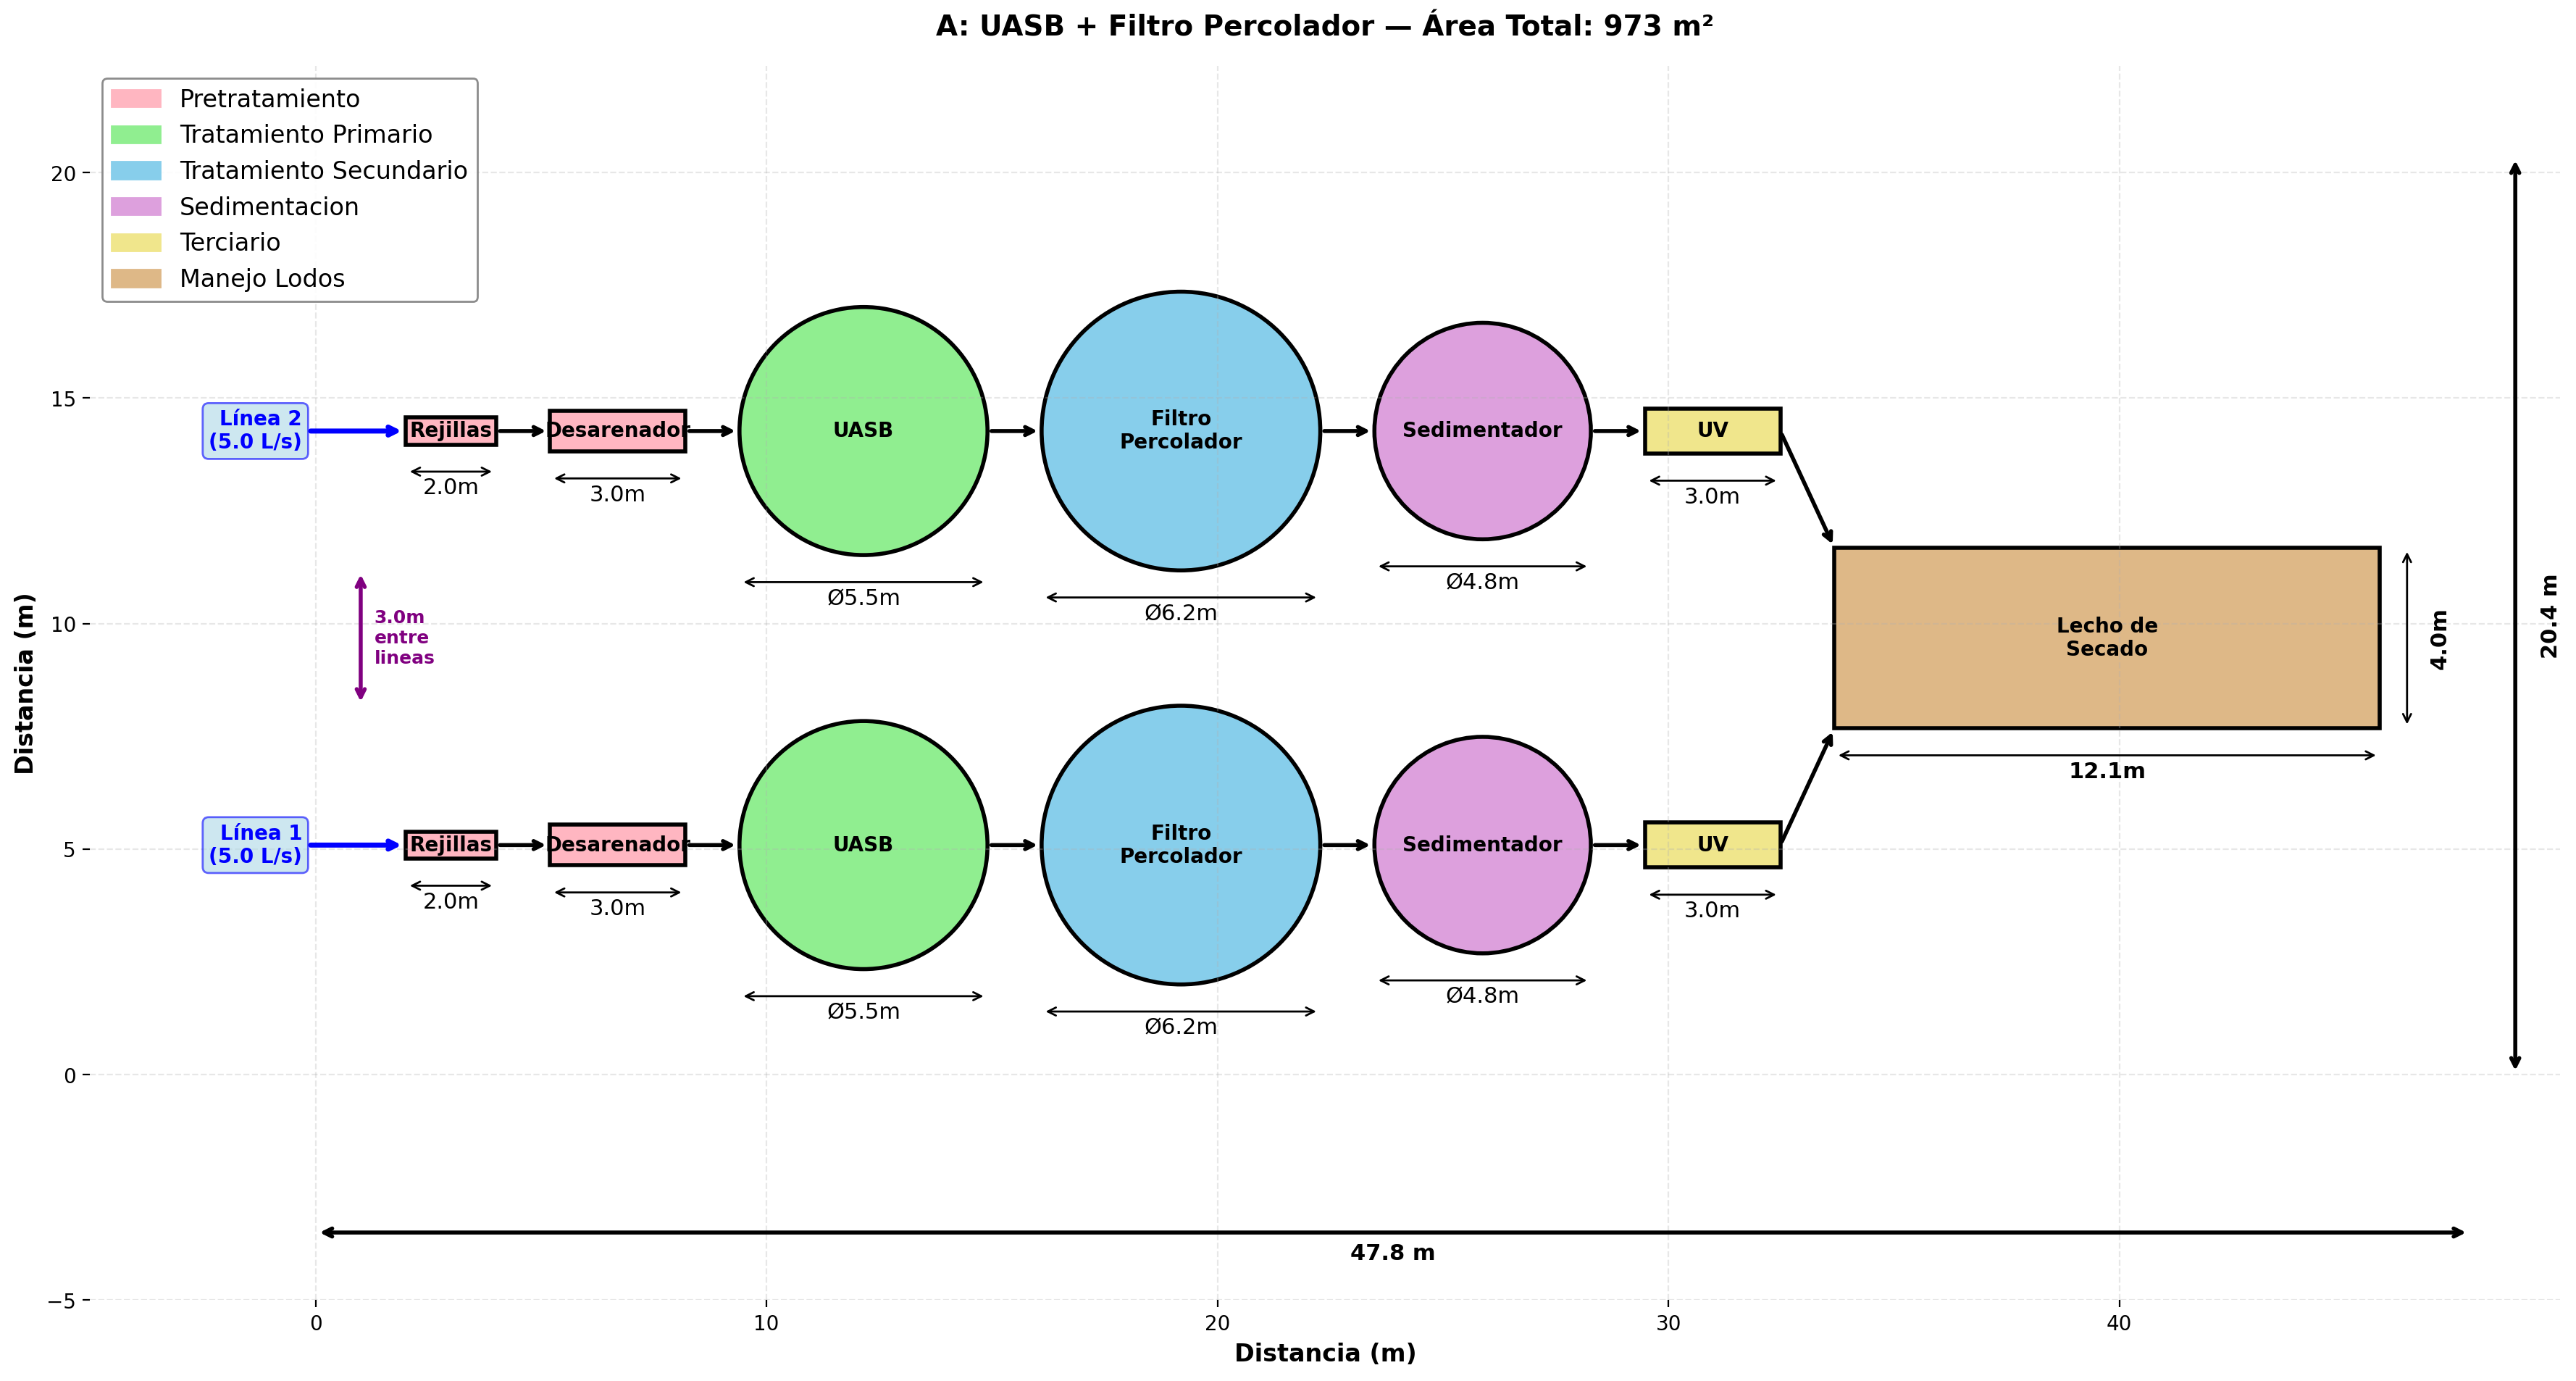
\includegraphics[width=\textwidth]{Layout_A_2lineas.png}
\caption{Disposición espacial de unidades - Alternativa A}
\label{fig:layout_a}
\end{figure}

El área de tratamiento calculada (unidades mas margenes minimos) es de aproximadamente 917 m². Sin embargo, para una operacion adecuada se requieren areas complementarias adicionales.

\textbf{Areas complementarias requeridas}

El area calculada de 917 m$^2$ corresponde unicamente a las unidades de tratamiento con sus margenes minimos de acceso. Sin embargo, para garantizar una operacion segura y eficiente de la planta durante toda su vida util, es necesario prever espacios adicionales para acceso vehicular y peatonal de operarios y visitantes, almacenamiento seguro de productos quimicos y herramientas, realizacion de analisis de control de calidad in-situ, estacionamiento para personal y visitantes, circulacion interna de vehiculos de mantenimiento y retiro de lodos, separacion de limites con zonas verdes para control de olores, y espacios administrativos para control operativo. La siguiente tabla resume las areas complementarias necesarias:

\begin{table}[H]
\centering
\caption{Areas complementarias de la planta}
\small
\begin{tabular}{lp{8cm}c}
\toprule
Area & Descripcion & Dimension aprox. \\
\midrule
Zona de amortiguacion & Perimetral alrededor de unidades (2-3 m) para acceso y seguridad & +20\% area tratamiento \\
\addlinespace
Bodega de quimicos & Almacenamiento de hipoclorito y productos quimicos & 10--15 m$^2$ \\
\addlinespace
Laboratorio/control & Analisis de calidad del agua (DBO, SST, CF, pH) & 15--20 m$^2$ \\
\addlinespace
Caseta de operacion & Control, panel, escritorio, bano & 12--15 m$^2$ \\
\addlinespace
Area de lavado & Limpieza de equipos y herramientas & 8--10 m$^2$ \\
\addlinespace
Estacionamiento & Vehiculos del personal y visitantes (2-3 vehiculos) & 50--60 m$^2$ \\
\addlinespace
Zona de camiones & Acceso de camiones cisterna/retiro de lodo & 50--80 m$^2$ \\
\addlinespace
Caminos internas & Circulacion vehicular y peatonal (ancho 3--4 m) & 80--120 m$^2$ \\
\addlinespace
Acceso principal & Entrada, porton y caseta de guardia & 20--30 m$^2$ \\
\addlinespace
Bodega general & Herramientas, repuestos, EPP & 15--20 m$^2$ \\
\addlinespace
Zona carga de lodos & Carga/descarga de lodo deshidratado & 20--30 m$^2$ \\
\addlinespace
Area verde/buffer & Separacion de limites, revegetacion & 15\% area total \\
\bottomrule
\end{tabular}
\end{table}

\textbf{Area total estimada del predio}

Considerando el area de tratamiento (917 m$^2$), amortiguacion (20\%), complementarias operativas y zona verde (15\% del total):

\begin{equation}
A_{total} = \frac{A_{tratamiento} + A_{amortiguacion} + A_{complementarias}}{1 - 0.15}
\end{equation}

\begin{itemize}[noitemsep,leftmargin=2em]
    \item[$A_{tratamiento}$] = 917 m$^2$
    \item[$A_{amortiguacion}$] = 183 m$^2$ (20\%)
    \item[$A_{complementarias}$] = 280--340 m$^2$ (operativas)
\end{itemize}

\begin{equation}
A_{total} = \frac{917 + 183 + 310}{0.85} \approx \mathbf{1600 \text{--} 1900 \text{ m}^2} \approx \mathbf{0.16 \text{--} 0.19 \text{ ha}}
\end{equation}

\textbf{Nota:} El area total del predio debe ser de aproximadamente 1600--1900 m$^2$ (0.16--0.19 ha) para operacion adecuada con circulacion interna, estacionamiento y zonas verdes.



%============================================================================
\newpage
\section{Resumen Ejecutivo de Resultados}
%============================================================================

El presente resumen consolida los resultados del dimensionamiento de la Planta de Tratamiento de Aguas Residuales (PTAR) para un caudal de dise\~no de \textbf{10.0 L/s} (5.0 L/s por linea).

\subsection{Parametros de Dise\~no}

\begin{table}[H]
\centering
\caption{Parametros de entrada del sistema}
\begin{tabular}{lc}
\toprule
\textbf{Parametro} & \textbf{Valor} \\
\midrule
Caudal medio (Q) & 5.0 L/s (432.0 m$^3$/d) \\
DBO$_5$ afluente & 243.1 mg/L \\
DQO afluente & 498.0 mg/L \\
SST afluente & 156.0 mg/L \\
Temperatura & 25.6 °C \\
\bottomrule
\end{tabular}
\end{table}

\subsection{Dimensionamiento de Unidades}

\begin{table}[H]
\centering
\caption{Resumen de unidades de tratamiento}
\begin{tabular}{p{4.5cm}ccc}
\toprule
\textbf{Unidad} & \textbf{Dimensiones} & \textbf{Cantidad} & \textbf{Parametro Clave} \\
\midrule
Rejillas & 0.38 m $\times$ 0.40 m & 2 canales & Separacion: 25 mm \\
Desarenador & 0.42 m $\times$ 5.0 m & 1 unidad & TRH: 1.8 min \\
Reactor UASB & D = 5.76 m, H = 4.3 m & 2 unidades & CH: 48.0 m$^3$/m$^2\cdot$d \\
Filtro Percolador & D = 6.56 m & 2 unidades & Q$_A$ = 4.00 m$^3$/m$^2\cdot$h \\
Sedimentador Secundario & 3.5 m $\times$ 9.8 m & 1 unidad & v$_d$ = 1.5 m/d \\
Desinfeccion (Cloro) & Dosis: 4.0 mg/L & 1 tanque & CT = 15 mg$\cdot$min/L \\
Lecho de Secado & 69.0 m$^2$ & 2 lechos & Aplicacion: 120 kg SST/m$^2\cdot$a\~no \\
\bottomrule
\end{tabular}
\end{table}

\subsection{Balance de Calidad del Agua}

\begin{table}[H]
\centering
\caption{Evolucion de parametros de calidad a traves del tratamiento}
\begin{tabular}{lccccc}
\toprule
\textbf{Parametro} & \textbf{Afluente} & \textbf{Post-UASB} & \textbf{Post-FP} & \textbf{Post-Sed} & \textbf{Efluente} \\
\midrule
DBO$_5$ (mg/L) & 243.1 & 60.0 & 30.0 & 21.0 & 40.6 \\
DQO (mg/L) & 498.0 & 131.3 & 65.6 & 45.9 & 99.6 \\
SST (mg/L) & 156.0 & 58.4 & 35.0 & 3.7 & 3.7 \\
CF (NMP/100mL) & 5e+06 & 2e+06 & 1e+06 & 5e+05 & 2526 \\
\midrule
\textbf{Remocion total} & -- & \textbf{65\%} & \textbf{40\%} & \textbf{30\%} & \textbf{83\%} \\
\bottomrule
\end{tabular}
\end{table}

\subsection{Verificacion de Cumplimiento Normativo}

\begin{table}[H]
\centering
\caption{Comparacion con limites de la TULSMA (Decreto 2132/2016)}
\begin{tabular}{lcccc}
\toprule
\textbf{Parametro} & \textbf{Efluente} & \textbf{Limite} & \textbf{Cumple} & \textbf{Margen} \\
\midrule
DBO$_5$ (mg/L) & 40.6 & 100 & \textcolor{green}{\textbf{S\'I}} & 59.4 mg/L \\
DQO (mg/L) & 99.6 & 250 & \textcolor{green}{\textbf{S\'I}} & 150.4 mg/L \\
SST (mg/L) & 3.7 & 100 & \textcolor{green}{\textbf{S\'I}} & 96.3 mg/L \\
CF (NMP/100mL) & 2526 & 3,000 & \textcolor{green}{\textbf{S\'I}} & 474 NMP/100mL \\
\bottomrule
\end{tabular}
\end{table}

\textbf{Conclusion:} El sistema dise\~nado cumple satisfactoriamente con todos los limites establecidos por la normativa colombiana para descargas a cuerpos de agua de uso recreativo con contacto indirecto (Clase 3).

\subsection{Requerimientos de Terreno}

\begin{table}[H]
\centering
\caption{Resumen de areas requeridas}
\begin{tabular}{lc}
\toprule
\textbf{Concepto} & \textbf{Area} \\
\midrule
Area de tratamiento & 917 m$^2$ \\
Area de amortiguacion (20\%) & 183 m$^2$ \\
Area complementaria operativa & 310 m$^2$ \\
Zona verde (15\% del total) & 138 m$^2$ \\
\midrule
\textbf{Area total requerida} & \textbf{917--1900 m$^2$ (0.16--0.19 ha)} \\
\bottomrule
\end{tabular}
\end{table}

\subsection{Produccion de Lodos}

\begin{table}[H]
\centering
\caption{Generacion y manejo de lodos}
\begin{tabular}{lc}
\toprule
\textbf{Concepto} & \textbf{Valor} \\
\midrule
Produccion lodos UASB & 6.4 kg SST/d \\
Produccion humus FP + Sed & 7.4 kg SST/d \\
\midrule
\textbf{Total lodos a manejar} & \textbf{13.8 kg SST/d} \\
Area de lechos de secado & 69.0 m$^2$ (2 unidades) \\
Frecuencia de aplicacion & 1 vez cada 3--4 meses \\
\bottomrule
\end{tabular}
\end{table}

\subsection{Consumos Estimados}

\begin{table}[H]
\centering
\caption{Consumos de energia y productos quimicos}
\begin{tabular}{lcc}
\toprule
\textbf{Concepto} & \textbf{Consumo} & \textbf{Unidad} \\
\midrule
Potencia electrica estimada & 5--8 & kW \\
Consumo energia & 40,000--60,000 & kWh/a\~no \\
Hipoclorito de sodio (12\%) & 17.7 & L/d \\
Consumo hipoclorito anual & 6 & m$^3$/a\~no \\
\bottomrule
\end{tabular}
\end{table}

\vspace{1cm}

\begin{center}
\fbox{
\begin{minipage}{0.9\textwidth}
\centering
\textbf{RESUMEN EJECUTIVO}\\[0.5em]
La PTAR Alternativa A (UASB + Filtro Percolador) para 10.0 L/s\\
requiere un area total de \textbf{0.16--0.19 ha} y produce un efluente que\\
cumple con la \textbf{TULSMA} para descarga a cuerpos de agua Clase 3.
\end{minipage}
}
\end{center}


\newpage
%============================================================================
% BIBLIOGRAFÍA
%============================================================================
\begin{thebibliography}{9}

\bibitem{metcalf2014}
Metcalf \& Eddy, AECOM. (2014).
\textit{Wastewater Engineering: Treatment and Resource Recovery}, 5th ed.
McGraw-Hill Education.

\bibitem{vanhaandel1994}
Van Haandel, A.C., \& Lettinga, G. (1994).
\textit{Anaerobic Sewage Treatment: A Practical Guide for Regions with a Hot Climate}.
John Wiley \& Sons.

\bibitem{sperling2007}
Sperling, M.V. (2007).
\textit{Biological Wastewater Treatment} (Vols. 1-6).
Departamento de Engenharia Sanitaria e Ambiental, UFMG.

\bibitem{wef2010}
Water Environment Federation. (2010).
\textit{WEF Manual of Practice No. 8: Design of Municipal Wastewater Treatment Plants}, 5th ed.
WEF Press.

\bibitem{romero2004}
Romero Rojas, J.A. (2004).
\textit{Tratamiento de Aguas Residuales: Teoría y Principios de Diseño}.
Editorial Escuela Colombiana de Ingeniería.

\bibitem{ops2005}
OPS/CEPIS. (2005).
\textit{Guía para el Diseño de Sistemas de Tratamiento de Aguas Residuales en Zonas Rurales y Pequeñas Comunidades}.
Organización Panamericana de la Salud.

\bibitem{kadlec2009}
Kadlec, R.H., \& Wallace, S.D. (2009).
\textit{Treatment Wetlands}, 2nd ed.
CRC Press.

\end{thebibliography}

\end{document}
